\documentclass[12pt, french]{article}

\usepackage{fancyhdr, fancybox, mathrsfs,lastpage}
\usepackage[most]{tcolorbox}
\usepackage[a4paper, margin={0.3in, .75in}]{geometry}
\usepackage{wrapfig}
\pagestyle{fancy}
\renewcommand\headrulewidth{1pt}
\renewcommand\footrulewidth{1pt}
\fancyhf{}
\rhead{ \em{Zakaria Haouzan}}
\lhead[C]{\em{2ème année baccalauréat Sciences mathématiques}}
\chead[C]{}
\rfoot[C]{}
\lfoot[R]{}
\cfoot[]{\em{Page \thepage / \pageref{LastPage}}}


\newtcolorbox{Box2}[2][
enhanced,
breakable
]{
                lower separated=false,
                colback=white,
colframe=white!20!black,fonttitle=\bfseries,
colbacktitle=white!30!gray,
coltitle=black,
enhanced,
attach boxed title to top left={yshift=-0.1in,xshift=0.15in},
title=#2,#1}


\begin{document}

\begin{center}

\vspace{-2cm}
   \shadowbox {\bf{ Oscillations forcées dans le circuit RLC }}
\end{center}

\vspace{-0.5cm}
%%_________________________Exercice ! :"_________________________Exercice
   \begin{Box2}{Exercice 1 : }
	   \begin{wrapfigure}[0]{r}{0.4\textwidth}
  \begin{center}
	  \vspace{-0.6cm}
	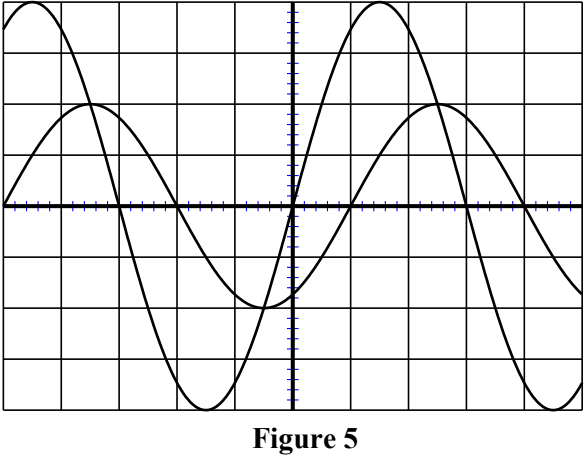
\includegraphics[width=0.4\textwidth]{./img/fig00RLCf.png}
  \end{center}
\end{wrapfigure}

On réalise un circuit série comportant :

\begin{itemize}
  \item  Un générateur (GBF) délivrant une tension \\alternative sinusoïdale
$u_m(t)= U_m cos(2\pi.N.t)$ \\de fréquence N.
\item  Le conducteur ohmique de résistance $R =150\Omega$
\item La bobine $b_1$
\item Un condensateur de capacité $C_0$

\end{itemize}

On visualise à l’aide d’un oscilloscope bi-courbe :
\begin{itemize}
  \item la tension $u(t)$ sur la voie $Y_A$.
  \item la tension $u_R(t)$ aux bornes du conducteur ohmique sur la voie $Y_B$.
\end{itemize}

     On obtient les courbes de la figure 5.
     La sensibilité verticale pour les deux voies est :$1 V.div^{-1}$

\begin{enumerate}
  \item Schématiser le montage expérimental permettant de
visualiser les tensions $u(t)$ et $u_R (t)$ en indiquant les
connexions à l’oscilloscope. 
\item Déterminer l’impédance $Z$ du circuit
\item Calculer le facteur de puissance du circuit et déduire la valeur de la puissance électrique moyenne.
\end{enumerate}
\end{Box2}


\begin{Box2}{Exercice 2 :  }
   \begin{wrapfigure}[10]{r}{0.4\textwidth}
  \begin{center}
	  \vspace{-0.8cm}
	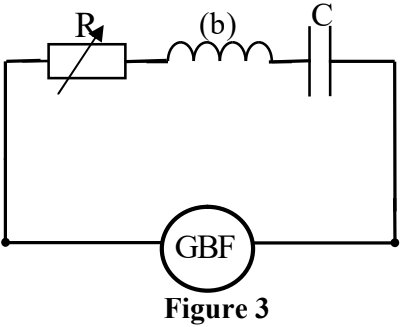
\includegraphics[width=0.3\textwidth]{./img/fig01RLCf.png}
	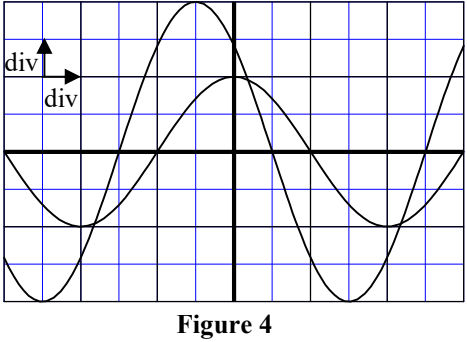
\includegraphics[width=0.4\textwidth]{./img/fig02RLCf.png}
  \end{center}
\end{wrapfigure}

On constitue un dipôle (D) par l'association en série de la bobine (b), du condensateur de capacité C et du conducteur ohmique de résistance R ajustée sur la valeur $R $=$ R_2 $=$ 20\,\Omega$. Le dipôle (D) est soumis à une tension alternative sinusoïdale fournie par un générateur GBF (Figure 3).

Un oscilloscope bicourbe est branché de manière à visualiser :
\begin{itemize}
    \item sur la voie A la tension $u(t) = U_m\cos(2\pi N t + \varphi_1)$ aux bornes du dipôle (D)
    \item sur la voie B la tension $u_R(t)$ aux bornes du conducteur ohmique
\end{itemize}

Données :
\begin{itemize}
    \item Base de temps : $0,5\,\text{ms}\cdot\text{div}^{-1}$
    \item La sensibilité verticale pour les deux voies A et B : $2\,\text{V}\cdot\text{div}^{-1}$
\end{itemize}

L'expression de l'intensité du courant électrique dans le circuit est :
\[ i(t) = I_m\cos(2\pi N t + \varphi_2) \]

Pour une fréquence N, on obtient l'oscillogramme de la figure 4.

\begin{enumerate}
    \item Faire le schéma du montage permettant de visualiser les deux tensions $u(t)$ et $u_{R}(t)$. 
    
    \item Déterminer les valeurs des grandeurs suivantes :
    \begin{enumerate}
      \item[a-] la fréquence N
      \item[b-] l'impédance Z du dipôle (D)
      \item[c-] $\Delta \varphi = \varphi_2 - \varphi_1$
    \end{enumerate}
    
    \item Calculer la puissance électrique moyenne consommée par le dipôle (D).
\end{enumerate}
\end{Box2}

\begin{Box2}{Exercice 3 :  }
On alimente un circuit, formé par la bobine, le résistor et l'un des deux condensateurs $C=120\mu F$ précédents utilisés, par un générateur GBF délivrant une tension alternative sinusoïdale de fréquence N variable et d'amplitude constante $U_m = 100~V$.


On ajuste l'inductance L sur la valeur $L_1 = 2,5~mH$ et la résistance R sur une valeur $R_1$.

Pour une fréquence $N_0$, la valeur efficace de l'intensité du courant est maximale : $I_0 \approx 0,71~A$.

Pour les fréquences $N_1 = 6,54~kHz$ et $N_2 = 12,90~kHz$, cette intensité est : $I_{eff} = 0,50~A$.

\begin{enumerate}
  \item Déterminer la fréquence $N_0$. 
  \item Vérifier que N1 et N2 délimitent la bande passante à –3dB et déduire la valeur du facteur de qualité Q.
  \item Calculer la valeur de $R_1$.
  \item Calculer, à la résonance, la puissance moyenne dissipée par effet Joule.
\end{enumerate}
\end{Box2}




\begin{center}

\vspace{-0.7cm}
   \Large{ \em{Exercices Supplémentaires}}
\end{center}

\vspace{-0.7cm}





%%_________________________Exercice !2 :"_________________________Exercice
\begin{Box2}{Exercice 4 : }

   \begin{wrapfigure}[10]{r}{0.4\textwidth}
  \begin{center}
	  \vspace{-0.8cm}
	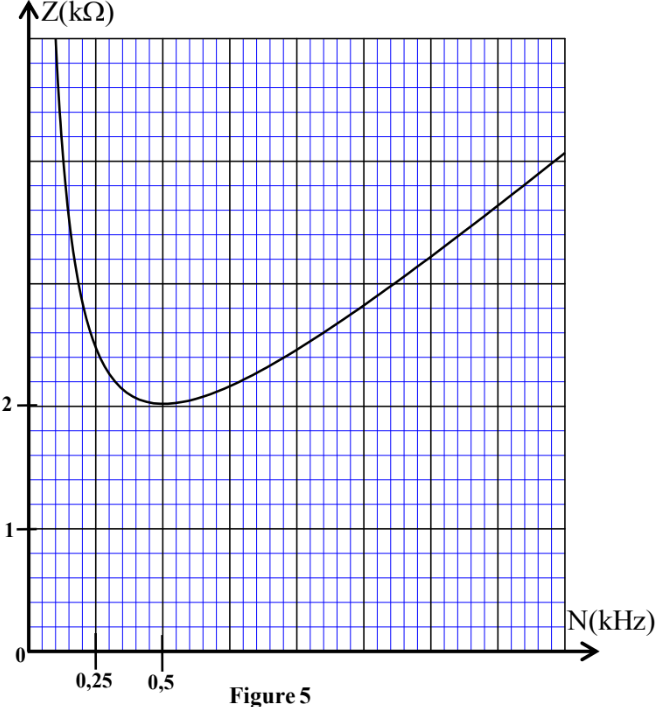
\includegraphics[width=0.4\textwidth]{./img/fig03RLCf.png}
  \end{center}
\end{wrapfigure}

On réalise un circuit RLC série comprenant:
\begin{itemize}
    \item un générateur délivrant une tension alternative sinusoïdale $u(t)$ de tension efficace constante et de fréquence $N$ réglable;
    \item un conducteur ohmique de résistance $R_3 = 1980\:\Omega$;
    \item la bobine (b) précédente;
    \item un condensateur de capacité $C_1$.
\end{itemize}

L'étude expérimentale a permis de tracer la courbe représentant les variations de l'impédance $Z$ du dipôle RLC en fonction de la fréquence $N$ (figure 5).

On prendra: $\pi = 3,14$ et $\pi^2 = 10$.

\begin{enumerate}
    \item Déterminer la fréquence de résonance.
    
    \item Calculer la capacité $C_1$ du condensateur.
    
    \item On note $I_0$ la valeur maximale de l'intensité efficace $I$ du courant dans le circuit. Pour $I = \frac{I_0}{\sqrt{2}}$, trouver la relation entre l'impédance $Z$ du circuit, $R_3$ et $r$.
    
    Déduire graphiquement la largeur de la bande passante à -3dB.
\end{enumerate}



\end{Box2}

\end{document}
